\documentclass[12pt, centerh1]{article}
\textwidth=165mm \headheight=0mm \headsep=10mm \topmargin=-10mm
\textheight=230mm %\footskip=1.5cm
\oddsidemargin=0mm
%\documentclass[12pt,letterpaper]{article}
%\usepackage[margin=1in]{geometry}
\RequirePackage[colorlinks,citecolor=blue,urlcolor=blue]{hyperref}
\usepackage{amsmath, amssymb,natbib}
%\usepackage[mathscr]{euscript}
%\usepackage{mathrsfs}
\usepackage{graphicx,bm}
\usepackage{color}
\usepackage{subcaption}
\usepackage{subcaption}
\usepackage[table]{xcolor}
\usepackage{longtable}
\usepackage{amsthm}
\usepackage[mathscr]{euscript}
\usepackage{relsize}
\usepackage{amsmath,tabularx}
\newcolumntype{P}[1]{>{\centering\arraybackslash}p{#1}}
\usepackage{rotating}
\usepackage{eurosym}
\usepackage{colonequals}
\usepackage{bbm}
\usepackage{lscape}
\usepackage{natbib}

%%% make comments using the following setup %%
% type \your name {comment}, 
% e.g. \sophie{i love lyme disease}
\newcommand{\bruce}[1]{{\textcolor{blue}{$\langle$BC: #1$\rangle$}}}
\newcommand{\sophie}[1]{{\textcolor{purple}{$\langle$SS: #1$\rangle$}}}
\newcommand{\lauren}[1]{{\textcolor{cyan}{$\langle$LF: #1$\rangle$}}}
\newcommand{\geneva}[1]{{\textcolor{red}{$\langle$GL: #1$\rangle$}}}
\newcommand{\thanesh}[1]{{\textcolor{yellow}{$\langle$TR: #1$\rangle$}}}

\title{We care about acaricide $<3$}

%%% put in alphabetical order
\author{\qquad name$^{1,3}$ \qquad\  name$^{1}$ \qquad\  name$^{1,3}$ \\  name$^{2}$ \quad\ Sophie Stelmach$^{1}$}

\date{{\small $^1$ Department of Mathematics \& Statistics, McMaster University, Ontario, Canada.\\[-6pt]
$^2$ add your institution\\[-6pt]
$^3$ \\[-6pt]
}
}
\linespread{1.5}
\pdfminorversion=4

\begin{document}

% makes title
\maketitle



\section{Introduction}
Lyme disease is a highly emerging vector-borne disease in North America, which is caused by the bacterium \textit{Borrelia} and transmitted via infected bites of black-legged ticks (\textit{Ixodes}) \citep{govcan}. The risk of disease is further propagated by the changes in migratory patterns northward of these ticks by climate change.

\subsection{Tick-host relationships}
\textbf{\textit{Borrelia}}, particularly B. burgdorferi sensu lato

\textbf{Black-legged tick}
I. scapularis is primary cause of LD in Eastern North America. I. scapularis is also a vector for many types of pathogens such as Borrelia mayonni, Powassan virus and Anaplasma phaocytophilum \citep{paulson2023multiomics}. This shows that besides Lyme disease, the black-legged tick can also increase the risk for poly microbial infections. 

\subsection{Biology of Lyme disease}

\textbf{Lyme disease}
Lyme disease clinical manifestation can be divided into three stages; early localization, early dissemination and late persistence. 

\textbf{Lyme disease in Canada}
A study in eastern and southern Ontario, Canada found \textit{Borrelia} sp in approximately 70 percent of ticks with a relative abundance of 0.01 percent \citep{clow2018microbiota}. Concentration of adult \textit{I. scapularis} carrying endosymbiotic and pathogenic microorganisms in southeastern Ontario \citep{paulson2023multiomics}. 

In this study, a mathematical model was developed to evaluate the efficacy of acacides as a Lyme disease intervention during the tick larval growth stage in Ontario, Canada.



\begin{figure}[h]
    \centering
    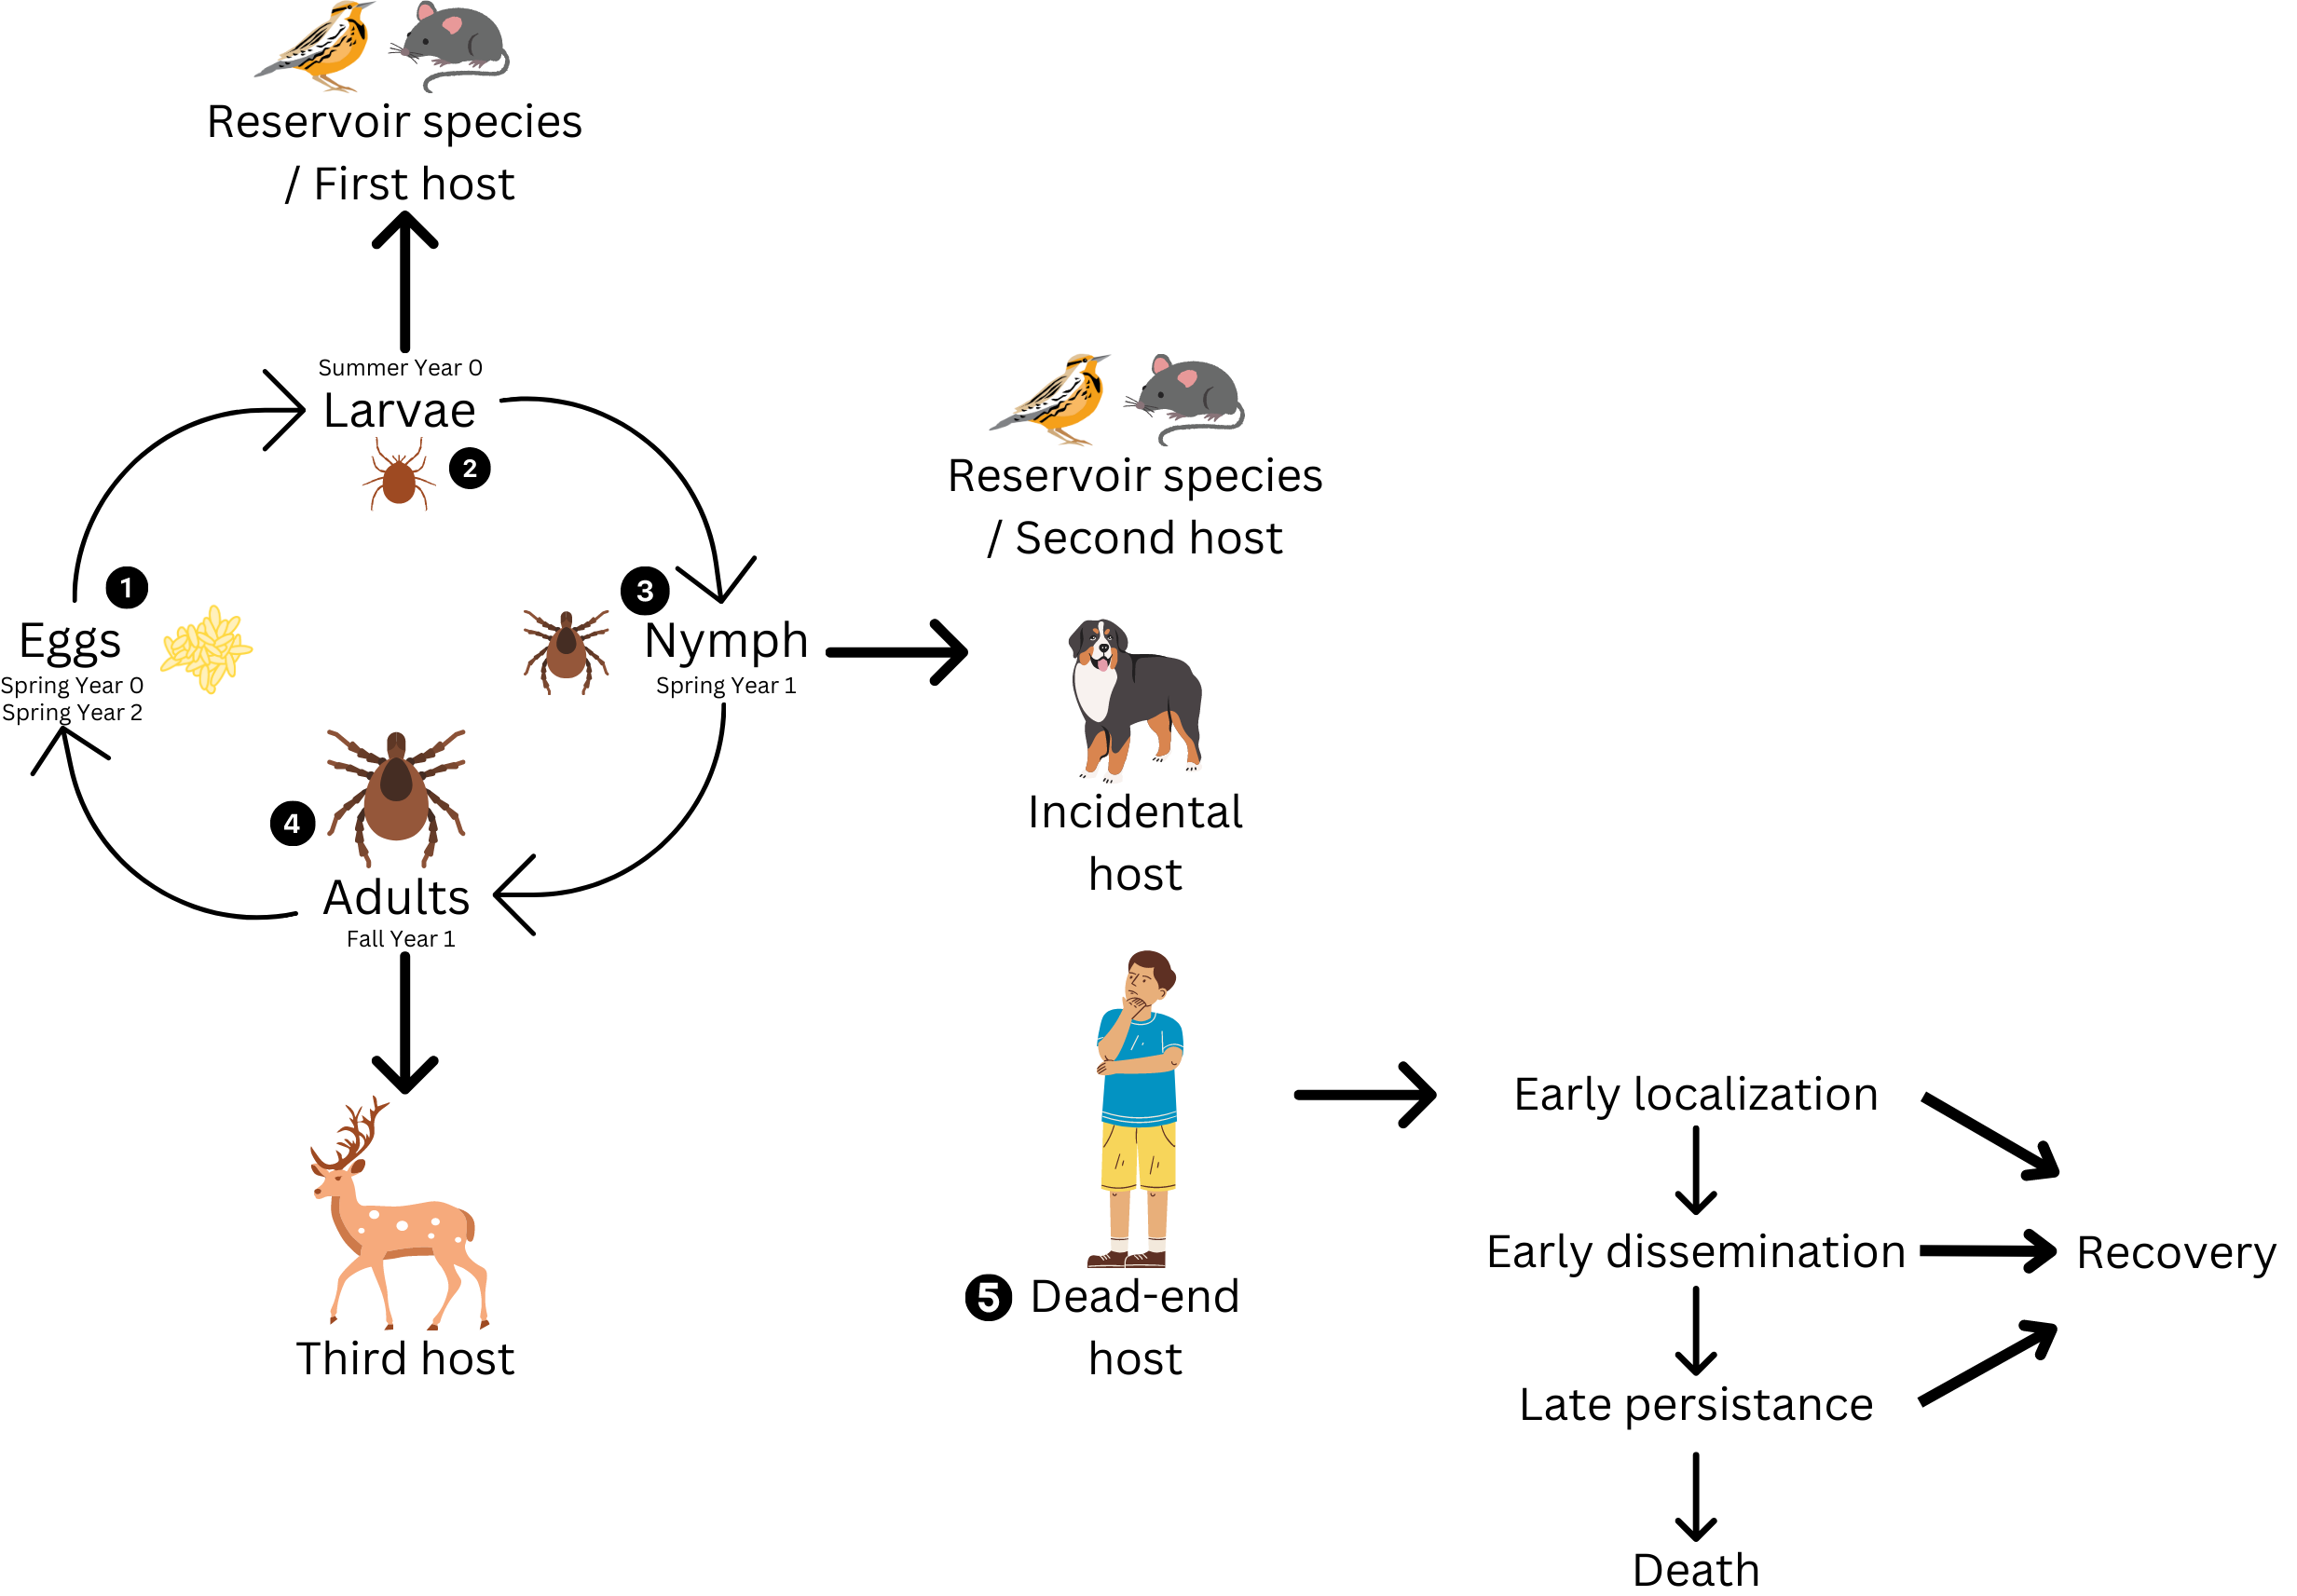
\includegraphics[scale = 0.15]{figures/Tick life cycle and progression of lyme disease.png}
    \caption{Diagram of tick life cycle and host bias.}
    \label{fig:lifecycle}
\end{figure}

\section{Methods}

\subsection{Proposed model}
The model proposed by \citet{lou2014tick} describes the tick life cycle and disease transmission between the tick and its hosts. The model features compartments that represent the various stages of the tick life cycle, including healthy ticks and infected ticks. We will base our analysis on this model, adding an intervention to prevent Lyme disease spread.

Ticks feed on their hosts in the larva, nymph, and adult stages of the life cycle, but only pose a risk to humans in the late larval and early-to-mid nymph stage. During the larval and nymph stage, ticks will feel on small rodents, at which point they risk acquiring Lyme disease-causing bacteria \sophie{cite}. Larvae, nymphs and adults feed on their hosts at different rates, which is why the model features different feeding rates for each of these stages. 

At each stage of the tick life cycle, we feature a mortality rate based on the values listed in \citet{lou2014tick}, which were found in previous publications. 


\sophie{Lauren/whoever insert compartmental diagram here}

\subsection{Rodent bait intervention}

\geneva{for now let's say S = susceptible, I = infected, P = poisonous}

Tick classes:
\begin{align}
    \frac{dL(t)}{dt} &= \left[b \,F_A \left(1 - \frac{R_P(t)}{R_S(t) + R_I(t) + R_P(t)}\right) - \frac{1}{K} A(t)\right]A(t) - (F_L + \mu_L) \,L(t) \\
    \frac{dN_S(t)}{dt} &= F_L\frac{R_S(t)}{R_S(t) + R_I(t) + R_P(t)}\,L(t) + (1-\beta_L)\,F_L \,L(t) \frac{R_I(t)}{R_S(t) + R_I(t) + R_P(t)} - (F_N - \mu_N) \,N_S(t) \\
    \frac{dN_I(t)}{dt} &= \beta_L F_L \,L(t) \frac{R_I(t)}{R_S(t) + R_I(t) + R_P(t)} - (F_N - \mu_N) \,N_I(t) \\
    \frac{dA_S(t)}{dt} &= F_N\frac{R_S(t)}{R_S(t) + R_I(t) + R_P(t)}\,N_S(t) - \mu_A \,A_S(t) \\
    \frac{dA_I(t)}{dt} &= F_N\left(1-\frac{R_P(t)}{R_S(t) + R_I(t) + R_P(t)}\right)\,N_I(t) + \beta_N \,F_N \,N_S(t) \, \frac{R_I(t)}{R_S(t) + R_I(t) + R_P(t)} - \mu_A \,A_I(t)
\end{align}

Rodent classes: \geneva{fix me later}
\begin{align}
    \frac{dR_S(t)}{dt} &= -\beta_R F_N \,\frac{R_S(t)}{R_S(t) + R_I(t) + R_V(t)} \,N_I - \nu R_S(t) - \mu_R R_S(t) \\
    \frac{dR_I(t)}{dt} &= \beta_R F_N \,\frac{R_S(t)}{R_S(t) + R_I(t) + R_V(t)} \,N_I(t) - \nu R_I(t) - \mu_R R_I(t) \\
    \frac{dR_P(t)}{dt} &= \nu (R_S(t) + R_I(t)) - \mu_R R_P(t)
\end{align}

\subsection{Model assumptions}
- assumptions
- dynamics?

Similarly to \citet{lou2014tick}, we assume that adult ticks feed only on deer, and that larvae and nymph ticks feed on rodents. We will assume that these are the only tick hosts in the environment.

\geneva{Extended model assumptions: 100\% efficacy and no waning immunity/half-life, infected rodents stay infected forever unless they take the bait (``neutralise" the infection)}

\begin{table}[h!]
\centering
 \begin{tabular}{||l l||} 
 \hline
 Parameter & Description \\ [0.5ex] 
 \hline\hline
 $M$ & The total number of rodents\\ 
 $D$ & The total number of the deer\\
 $F_L$ & The rate at which larval ticks attach on rodents. This is a function of M\\
 $F_N$ & The rate at which nymphal ticks bite rodents. This is a function of M\\ 
 $F_A$ & The rate at which adult ticks attack deer. This is a function of D\\
 $b$ & The larvae hatching per adult tick–deer interaction in the absence
of tick self-regulation\\
 $1/K$ & The scale of self-regulation in tick reproduction\\
 $\mu_L$ & The death rate for larval ticks\\
 $\mu_N$ & The death rate for nymphal ticks\\
 $\mu_A$ & The death rate for adult ticks\\
 $\beta_L$ & Transmission coefficient of spirochete infection to rodents\\
 $\beta_N$ & Transmission coefficient of spirochete infection to larval ticks\\
 $\beta_A$ & Transmission coefficient of spirochete infection to nymphal ticks\\[1ex] 
 \hline
 \end{tabular}
\end{table}



\section{Results}



\section{Discussion}

\subsection{Model Implications}

\subsection{Effect on Policy Decisions}

\subsection{Future Studies}


\section{Conclusion}



\newpage
\bibliographystyle{chicago} %idk what style we want to do
\bibliography{bib}
\end{document}
